\documentclass[10pt]{beamer}

\usetheme{metropolis}
\usepackage{appendixnumberbeamer}

\usepackage{booktabs}
\usepackage[scale=2]{ccicons}
\usepackage{graphicx}
\usepackage{hyperref}
\usepackage{circuitikz}
\usepackage{pdflscape}
\usepackage{smartdiagram}

\usepackage{color}
\usepackage{listings}

\lstset{
	basicstyle=\footnotesize\ttfamily,
    keepspaces=true,
    showstringspaces=false,
    language=PHP,
    commentstyle=\ttfamily,
}

\usepackage[OT4]{polski}
\usepackage[utf8]{inputenc}

\usepackage{pgfplots}
\usepgfplotslibrary{dateplot}

\usepackage{xspace}
\newcommand{\themename}{\textbf{\textsc{metropolis}}\xspace}

\setbeamertemplate{frame footer}{}
\setbeamertemplate{frame numbering}{}

\usetikzlibrary{shapes,arrows}

\tikzstyle{decision} = [diamond, draw, fill=blue!20, 
    text width=4.5em, text badly centered, node distance=3cm, inner sep=0pt]
\tikzstyle{block} = [rectangle, draw, fill=blue!20, 
    text width=5em, text centered, rounded corners, minimum height=4em]
\tikzstyle{line} = [draw, -latex']
\tikzstyle{cloud} = [draw, ellipse,fill=red!20, node distance=3cm,
    minimum height=2em]


\title{Reaktywne aplikacje frontendowe}

\subtitle{Projektowanie i programowanie systemów internetowych I}
\author{mgr inż. Krzysztof Rewak}
\date{\today}
\institute{Wydział Nauk Technicznych i Ekonomicznych \\ Państwowa Wyższa Szkoła Zawodowa im. Witelona w Legnicy}

\begin{document}

\maketitle

\begin{frame}{Plan prezentacji}
  \setbeamertemplate{section in toc}[sections numbered]
  \tableofcontents[hideallsubsections]
\end{frame}


\section{Aplikacje frontendowe}

\begin{frame}{Frontend?}
	Frontendem będziemy nazywali graficzny interfejs użytkownika (GUI) aplikacji webowej. W dużym uproszczeniu możemy wydzielić między innymi warstwę \textbf{prezentacji} oraz warstwę \textbf{interakcji}.
	
	Pierwsza powinna przedstawiać dane przesłane z backendu aplikacji, druga - umożliwić zmianę tych danych.
\end{frame}

\begin{frame}{Frontend = HTML?}
	Najprostszy frontend? Będzie to zwykły HTML za pomocą którego można stworzyć praktycznie kompletny i funkcjonalny interfejs dla niektórych rozwiązań.
\end{frame}

\begin{frame}[fragile]{\texttt{index.html}}
	\begin{lstlisting}
<!DOCTYPE html>
<html lang="en">

  <head>
    <meta charset="utf-8">
    <title>Homepage title</title>
  </head>

  <body>
    <h1>Title</h1>
    <p>Content</p>
  </body>

</html>
	\end{lstlisting}
\end{frame}

\begin{frame}{Frontend != HTML}
	Niestety szybko może się okazać, że sam HTML nie wystarczy i do pracy będzie trzeba zaprzegnąć \emph{coś więcej}.
	
	Po stronie serwera można wygenerować interfejs użytkownika za pomocą PHP (do czego zresztą początkowo przecież powstał) lub systemów szablonów dla większości języków programowania. Można wówczas skorzystać z dobrodziejstw instrukcji warunkowych, pętli i innych konstrukcji języka, które zautomatyzują budowanie frontendu (chociażby list i tabel).
\end{frame}

\begin{frame}{Zrzućmy to na klienta}
	Z czasem modne stało się przerzucanie odpowiedzialności za renderowanie frontendu z serwera aplikacji na użytkownika.
	
	Ostateczną formą realizacji tej idei są SPA wykorzystające zewnętrzne API.
	
	Wszystko oczywiście za pomocą JavaScriptu i jego dialektów.
\end{frame}

\begin{frame}[fragile]{jQuery}
	\begin{lstlisting}
$loading = $("#loading");
$form = $("#user-form");
$button = $("#user-save-button");
$alertContent = $("#success-info > div");

$button.click(function() {
    $loading.show();

    url = "/api/user/" + $form.data("user-id");
    data = $form.serialize();
    
    $.post(url, data, function(response) {
        $loading.hide();
        $alertContent.html(response.message);
    });
});
	\end{lstlisting}
\end{frame}

\begin{frame}{jQuery}
	Jeszcze kilka lat temu biblioteka jQuery była najprawdopodobniej najpopularniejszym frontendowym rozwiązaniem w internecie. Wciąż jest masowo stosowana, jednakże powoli wypierają ją reaktywne frameworki.
\end{frame}

\section{Reaktywne aplikacje frontendowe}

\begin{frame}{Przegląd rozwiązań}
	Obecnie warto się zainteresować jednym z poniższych:
	\begin{itemize}
	\item Angular
	\item React
	\item Vue.js
	\end{itemize}
\end{frame}

\begin{frame}{Przegląd rozwiązań}
	Należy też na pewno wspomnieć o innych, może obecnie nieco mniej popularnych:
	\begin{itemize}
	\item Meteor
	\item Ember.js
	\item Backbone.js
	\item Aurelia
	\item Polymer
	\end{itemize}
\end{frame}

\begin{frame}{Reaktywność?}
	Jak należy rozumieć \emph{reaktywność} w aplikacji webowej?
\end{frame}

\begin{frame}[fragile]{Reaktywność?}
	Wyobraźmy sobie formularz z polem tekstowym, do którego użytkownik wpisuje wartość, którą chce znaleźć w tabeli poniżej.
	
	\begin{lstlisting}
<form id="search" method="POST" class="search form">
    <input
        class="standard full width text input"
        placeholder="Enter searching phrase..."
        value=""
        autofocus
    >
</form>

<table id="results" class="list table">
    <!-- (...) -->
</table>
	\end{lstlisting}
\end{frame}

\begin{frame}[fragile]{Reaktywność?}
	Korzystając z jQuery (lub nawet \emph{vanilla JS}, trzeba obserwować element DOM i reagować na jego zmiany:
	
	\ \\ \ \\

	\begin{lstlisting}
$input = $("#search > .text.input");
$table = $("#results");

$input.change(function(event) {
    $.get("/api/results?" + $(this).val(), function(response) {
        $table.empty();
        response.data.forEach(function(result) {
            $table.append("<tr><td>" + result + "</td></tr>");
        });
    });
});
	\end{lstlisting}
\end{frame}

\begin{frame}{Reaktywność?}
	Powyższe rozwiązanie działa, ale nie nazwałbym go dobrym. Ma też kilka mankamentów, między innymi:
	\begin{itemize}
	\item przy każdej zmianie w polu tekstowym pobiera nową listę wyników,
	\item za każdym razem czyści całą tabelę,
	\item miesza warstwy logiki biznesowej i prezentacji danych,
	\item zaczyna generować tzw. \emph{callback hell},
	\item i wiele innych.
	\end{itemize}
\end{frame}

\begin{frame}[fragile]{Reaktywność!}
	Poniżej mamy podobne formularz i tabelę, ale zbudowane przy pomocy Vue.js:
	
	\begin{lstlisting}
<div id="application">
    <form method="POST" class="search form">
        <input
            class="standard full width text input"
            placeholder="Enter searching phrase..."
            v-model="searchPhrase"
            autofocus
        >
    </form>

    <table class="list table">
       <tr v-for="result in results">
           <td>{{ result }}</td>
       </tr>
    </table>
</div>
	\end{lstlisting}
\end{frame}

\begin{frame}[fragile]{Reaktywność!}
	\begin{lstlisting}
export default {
    data() {
        return {
            fetchedResults: [],
            searchPhrase: "",
        }
    },
    computed: {
        results() {
            let phrase = this.searchPhrase
            return this.fetchedResults
                .filter(result => result.includes(phrase))
        }
    },
    mounted() {
        fetch("/api/results?" + this.searechPhrase)
            .then(response => {
                this.fetchedResults = response.data
            })
    }
}
	\end{lstlisting}
\end{frame}

\begin{frame}{Reaktywność!}
	Co widać?
	\begin{itemize}
	\item zmienna \texttt{searchPhrase} jest obserwowana przez Vue i przy zmianie wartości pola tekstowego nastąpi automatyczne filtrowanie uprzednio pobranych danych,
	\item tabela jest renderowana na bieżąco w zależności od wyników,
	\item rozdziela warstwy logiki biznesowej i prezentacji danych,
	\item wykorzystujemy tutaj \emph{arrow functions}, które między innymi zwiększają czytelność kodu.
	\end{itemize}
\end{frame}

\begin{frame}{Programowanie reaktywne}
	Programowanie reaktywne to jeden z paradygmatyów programowania. Do tej pory na wykładach rozmawialiśmy między innymi o programowaniu strukturalnym, obiektowym, funkcyjnym czy imperatywnym.
\end{frame}

\begin{frame}{Programowanie reaktywne}
	Programowanie reaktywne opiera się na reakcjach na zdarzenia, które z grubsza można podzielić na trzy typy: interakcje od strony użytkownika, odpowiedzi serwera oraz zdarzenia wewnętrzne, systemowe.
\end{frame}

\section{Interludium: JavaScript}

\begin{frame}{\emph{Java w wersji Script}}
	JavaScript jest obecnie jednym z najpopularniejszych, a jednocześnie jednym z najbardziej kochanych, znienawidzonych, nierozumianych, niedocenianych i przereklamowanych języków programowania.
	
	Sam wstęp dużo mówi o tym jakiego rodzaju to język.
\end{frame}

\begin{frame}{npm}
	Podstawą środowiska deweloperskiego dla programisty JS będą między innymi:
	\begin{itemize}
	\item Node.js, czyli środowisko uruchomieniowe;
	\item npm, czyli manager pakietów;
	\item webpack, czyli bundler modułów
	\item Babel, czyli kompilator/transpilator
	\end{itemize}
	
	... i masa innych programów, które co kilka miesięcy się zmieniają.
\end{frame}

\begin{frame}{Warto wiedzieć \#1: hot-reload}
	Korzystając z webpacka (ale także Grunta lub Gulpa) można skonfigurować projekt pod tzw. \emph{hot-reloading}. Wówczas każda zmiana kodu w naszym IDE zostanie odnotowana przez system, przetworzona oraz na żywo wyświetlona w oknie przeglądarki.
	
	Jedna z najwygodniejszych frontendowych funkcjonalności, którą warto zbadać.
\end{frame}

\begin{frame}[fragile]{Warto wiedzieć \#2: ES6}
	ES6, czyli ECMAScript 2016, to standard, który przyniósł wiele dobrego JavaScriptowi. Między innymi wprowadził funkcje strzałkowe, które upraszczają zapis, ale także zmienają zakres zmiennej \texttt{this}:

	\begin{lstlisting}
var self = this;
[4, 8, 15, 16, 23, 42].map(function(n) {
    return n * self.getMultiplier();
});
	\end{lstlisting}
	
	Na pewno wersja strzałkowa wygląda schludniej:

	\begin{lstlisting}
[4, 8, 15, 16, 23, 42].map(n => n * this.getMultiplier())
	\end{lstlisting}
\end{frame}

\begin{frame}[fragile]{Warto wiedzieć \#3: TypeScript}
	Jedną z najczęściej wytykanych wad JavaScriptu jest jego rzekoma nieprzewidywalność w ujęciu typowania. Dla takich ludzi stworzono TypeScript, który umożliwia statyczne typowanie:
	
	\ \\ \ \\

	\begin{lstlisting}
function sum(a, b) {
    return a + b
}
	\end{lstlisting}

	\begin{lstlisting}
function sum(a: number, b: number): number {
    return a + b
}
	\end{lstlisting}
\end{frame}

\begin{frame}{Warto wiedzieć \#3: TypeScript}
	\centering
	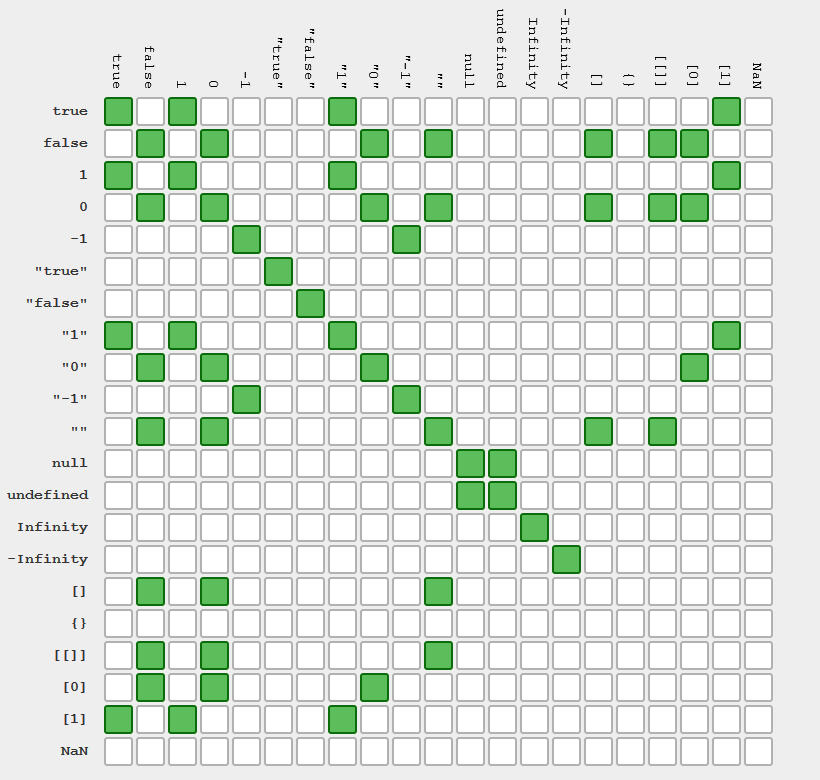
\includegraphics[width=.8\textwidth]{matrix.png}
\end{frame}

\section{Przegląd rozwiązań}

\begin{frame}{Angular}
	Angular, poprzednio AngularJS, to opracowany przez Google frontendowy framework i obecnie jedno z dwóch najpopularniejszych rozwiązań tego typu na świecie.
\end{frame}

\begin{frame}{Angular}
	\begin{itemize}
	\item wymaga TypeScriptu;
	\item model MVVM gwarantujący separację warstw;
	\item warstwa prezentacji danych oparta o ulepszony HTML;
	\item dwustronne wiązanie danych, a więcej reaktywne podejście;
	\end{itemize}
\end{frame}

\begin{frame}{Angular}
	\begin{itemize}
	\item posiada rozbudowany system wstrzykiwania zależności;
	\item gigantyczna społeczność i szczegółowa dokumentacja;
	\item każdy komponent definiuje się jako nowy folder z przynajmniej trzema plikami: \texttt{*.html},  \texttt{*.ts} i  \texttt{*.scss};
	\item nowe wersje wychodza stosunkowo bardzo często i bywają ze sobą niekompatybilne.
	\end{itemize}
\end{frame}

\begin{frame}{React}
	React to opracowany - tym razem - przez Facebooka frontendowy framework i obecnie również jedno z dwóch najpopularniejszych rozwiązań tego typu na świecie.
\end{frame}

\begin{frame}{React}
	\begin{itemize}
	\item reklamuje się jako biblioteka, nie framework;
	\item wykorzystuje Virtual DOM;
	\item bardzo lekki i szybki;
	\item wymaga bardziej zaawansowanej wiedzy na temat JavaScriptu;
	\item jednostronne wiązanie danych;
	\item korzystając z React Native można budować aplikacje mobilne;
	\end{itemize}
\end{frame}

\begin{frame}[fragile]{React}
	\begin{itemize}
	\item wykorzystuje JSX:
	\end{itemize}
	
	\begin{lstlisting}
const navigation = document.getElementById("navigation");

const user = {
    id: "cb0824c1-b88c-4965-b490-b6a9066aff44",
    name: "krewak"
};

const component = (
    <div>
        <i class="user icon"></i>
        { user.name }
    </div>
);

ReactDOM.render(welcomer, navigation);
	\end{lstlisting}
\end{frame}

\begin{frame}{Vue.js}
	Vue.js to opracowany głównie przez Evana You frontendowy framework i obecnie jedno z najbardziej rozwijających się rozwiązań tego typu.
\end{frame}

\begin{frame}{Vue.js}
	\begin{itemize}
	\item szczegółowa dokumentacja;
	\item niewiele waży;
	\item może być stosowane jako import z CDN-a dla jednego komponentu lub pełna SPA;
	\item korzysta z Virtual DOM;
	\end{itemize}
\end{frame}

\begin{frame}{Vue.js}
	\begin{itemize}
	\item jedno- i dwustronne wiązanie danych;
	\item udostępnia możliwość tworzenia tzw. Vue components
	\item umożliwia zmianę języków i dialektów dla szablonów, stylów i skryptów;
	\item uważany za najłatwiejszy do nauczenia się.
	\end{itemize}
\end{frame}

\section{Podsumowanie}

\begin{frame}{W prawdziwym świecie}
	\centering
	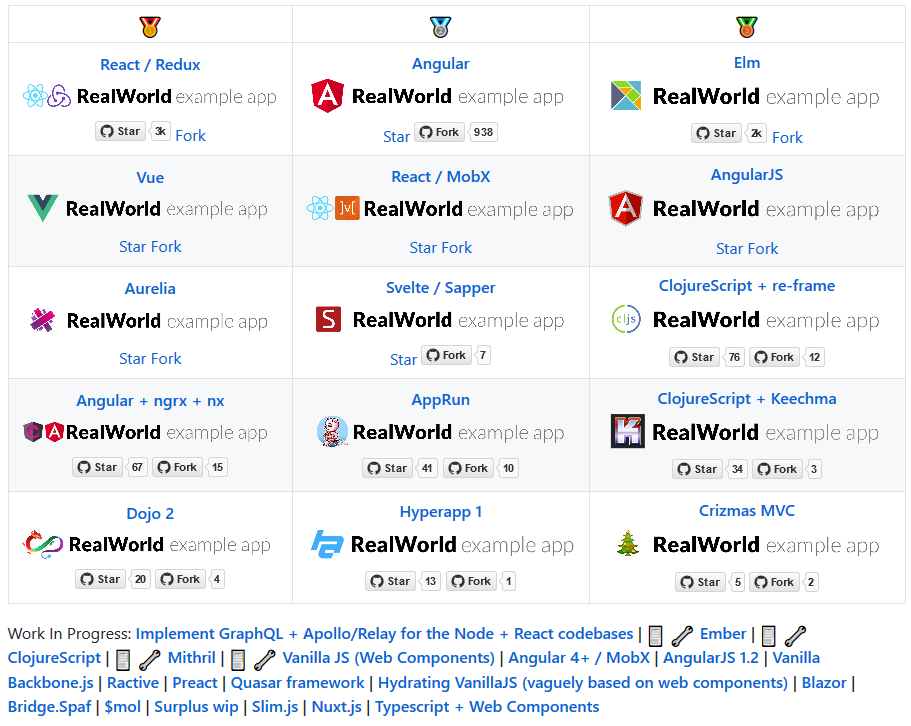
\includegraphics[width=.8\textwidth]{realworld.png}
\end{frame}

\begin{frame}{Bibliografia i ciekawe źródła}
  
	\begin{thebibliography}{9}
	
		\bibitem{realworld}
		\url{https://realworld.io/}
		- naprawdę warto!
		
		\bibitem{comp}
		\url{https://dzone.com/articles/react-vs-angular-vs-vuejs-a-complete-comparison-gu}
	
	\end{thebibliography}

\end{frame}

\appendix

\begin{frame}[standout]
	Pytania?
\end{frame}

\begin{frame}{}

	Kod prezentacji dostępny jest w repozytorium git pod adresem \texttt{https://bitbucket.org/krewak/pwsz-ppsi} \\ \ \\

	\begin{figure}
		\centering
		\href{https://bitbucket.org/krewak/pwsz-ppsi}{
			
\includegraphics[width=.15\textwidth]{../_template/bitbucket.png}
		}
	\end{figure}
	
	Wszystkie informacje dot. kursu dostępne są pod adresem \texttt{http://pwsz.rewak.pl/kursy/4} \\ \ \\

	\begin{figure}
		\centering
		\href{http://pwsz.rewak.pl/kursy/3}{
			
\includegraphics[width=.15\textwidth]{../_template/rewak.png}
		}
	\end{figure}

\end{frame}

\end{document}
